\documentclass{beamer}
\usepackage{tikz,amsmath,hyperref,graphicx,stackrel,animate,bm}
\usetikzlibrary{positioning,shadows,arrows,shapes,calc}
\newcommand{\argmax}{\operatornamewithlimits{argmax}}
\newcommand{\argmin}{\operatornamewithlimits{argmin}}
\mode<presentation>{\usetheme{Frankfurt}}
\AtBeginSection[]
{
  \begin{frame}<beamer>
    \frametitle{Outline}
    \tableofcontents[currentsection,currentsubsection]
  \end{frame}
}
\title{Lecture 15: Principal Components and Eigenfaces}
\author{Mark Hasegawa-Johnson\\These slides are in the public domain}
\date{ECE 417: Multimedia Signal Processing}  
\begin{document}

% Title
\begin{frame}
  \maketitle
\end{frame}

% Title
\begin{frame}
  \tableofcontents
\end{frame}

%%%%%%%%%%%%%%%%%%%%%%%%%%%%%%%%%%%%%%%%%%%%
\section[Review]{Review: Gaussians}
\setcounter{subsection}{1}

\begin{frame}
  \frametitle{Scalar Gaussian random variables}
  \[
  p_X(x) = \frac{1}{\sqrt{2\pi\sigma^2}}e^{-\frac{1}{2}\left(\frac{x-\mu}{\sigma}\right)^2}
  \]
  \centerline{\includegraphics[height=2in]{exp/gaussian_pdfs.png}}
  {\footnotesize\url{https://commons.wikimedia.org/wiki/File:Normal_Distribution_PDF.svg}}
\end{frame}

\begin{frame}
  \frametitle{Scalar Gaussian random variables}
  \[
  \mu=E[X],~~~\sigma^2=E[(X-\mu)^2]
  \]
  \centerline{\includegraphics[height=2in]{exp/gaussian_pdfs.png}}
  {\footnotesize\url{https://commons.wikimedia.org/wiki/File:Normal_Distribution_PDF.svg}}
\end{frame}

\begin{frame}
  \frametitle{Gaussian random vectors}
  \[
  p_{\mathbf{X}}(\mathbf{x})=\frac{1}{(2\pi)^{D/2}|\bm{\Sigma}|^{1/2}}e^{-\frac{1}{2}
    (\mathbf{x}-\bm{\mu})^T\bm{\Sigma}^{-1}(\mathbf{x}-\bm{\mu})}
  \]
  \centerline{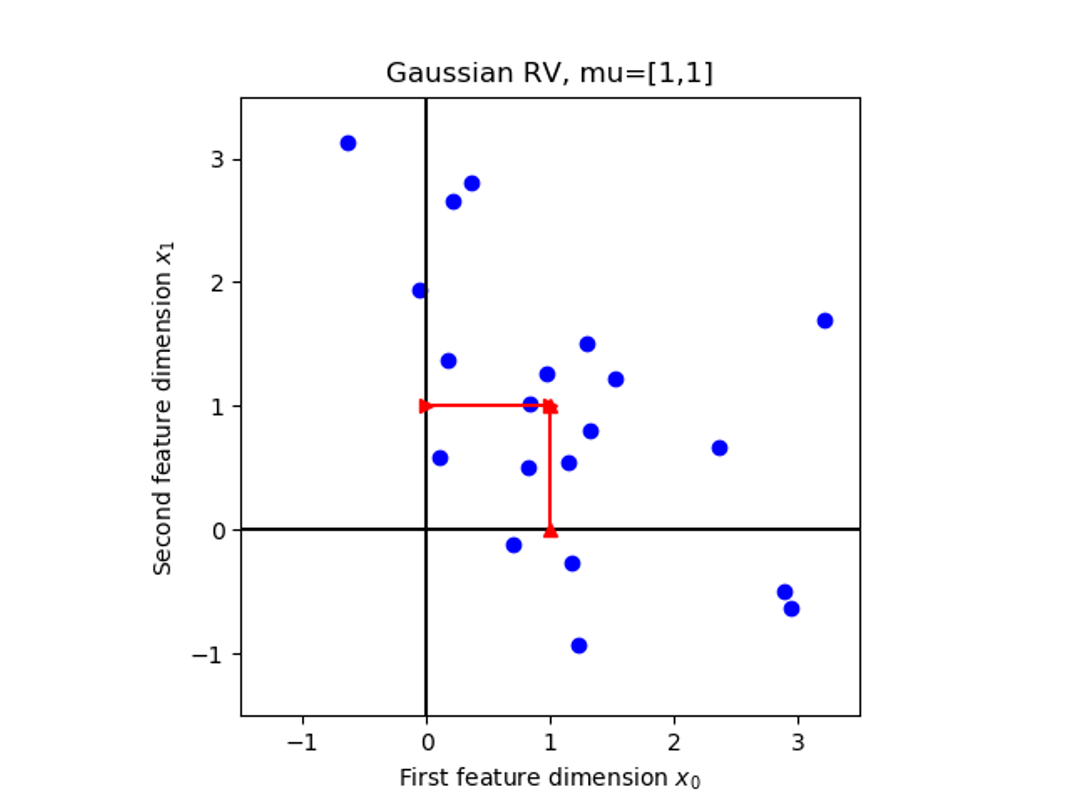
\includegraphics[height=2in]{exp/gaussian_vectors.png}}
  {\footnotesize\url{https://commons.wikimedia.org/wiki/File:EM-Gaussian-data.svg}}
\end{frame}

\begin{frame}
  \begin{columns}
    \column{2.125in}
    \begin{block}{Gaussian random vectors}
      \[
      \mathbf{x}=\left[\begin{array}{c}x_1\\\cdots\\x_{D}\end{array}\right]
      \]
      \[
      \bm{\mu}=E[\mathbf{x}]=\left[\begin{array}{c}\mu_1\\\cdots\\\mu_{D}\end{array}\right]
      \]
    \end{block}
    \column{2.125in}
    \begin{block}{Example: Instances of Gaussian random vectors}
      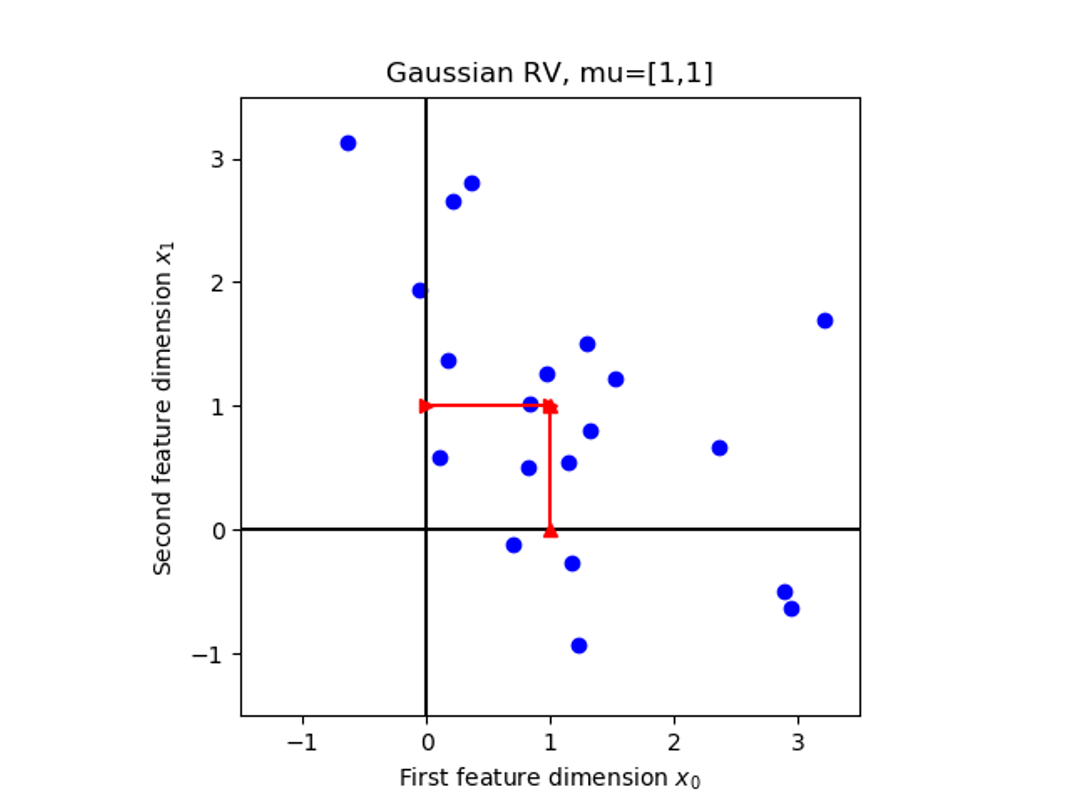
\includegraphics[width=\textwidth]{exp/gaussian_vectors.png}
      {\footnotesize\url{https://commons.wikimedia.org/wiki/File:EM-Gaussian-data.svg}}
    \end{block}
  \end{columns}
\end{frame}

\begin{frame}
  \begin{columns}
    \column{2.25in}
    \begin{block}{Gaussian random vectors}
      If the Gaussians are independent but not identical, then:
      \[
      \bm{\Sigma}= \left[\begin{array}{ccc}
          \sigma_1^2 & 0 & \cdots\\
          0 & \sigma_2^2 &  \cdots\\
          \vdots & \vdots &  \sigma_{D}^2\end{array}\right]
      \]
      where
      \[
      \sigma_{i}^2=E[(x_i-\mu_i)^2]
      \]
    \end{block}
    \column{2in}
    \begin{block}{Example: Instances of Gaussian random vectors}
      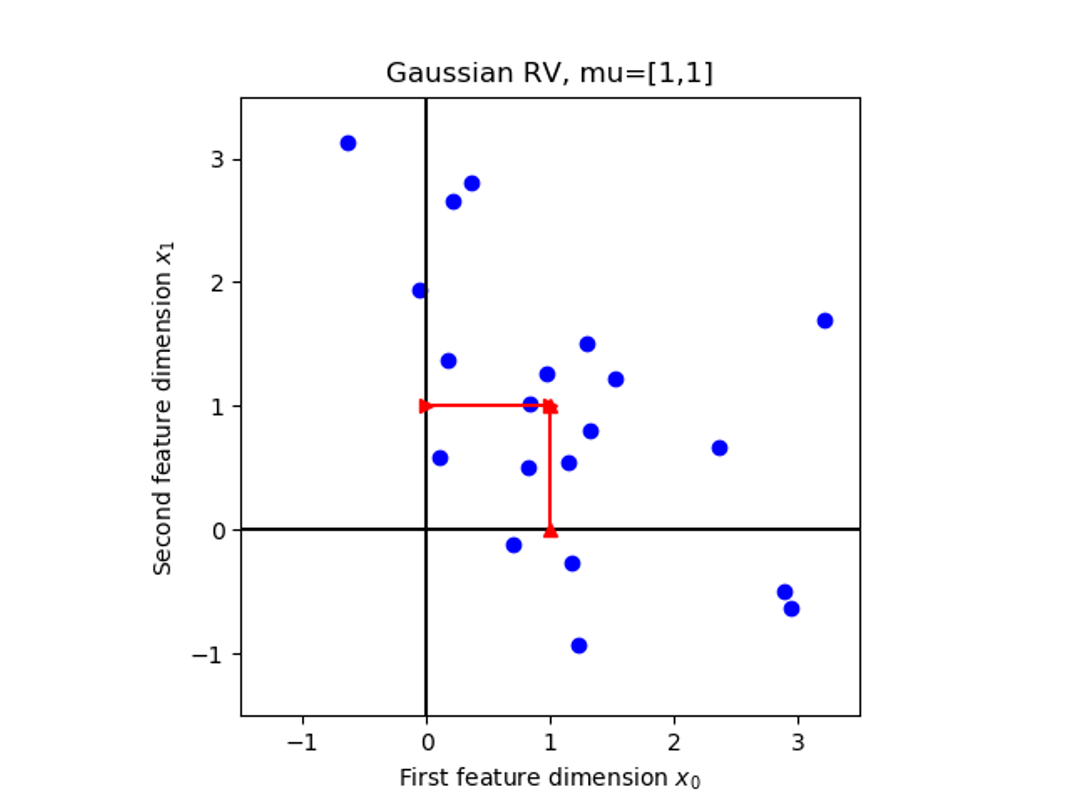
\includegraphics[width=1.9in]{exp/gaussian_vectors.png}
      {\footnotesize\url{https://commons.wikimedia.org/wiki/File:EM-Gaussian-data.svg}}
    \end{block}
  \end{columns}
\end{frame}

\begin{frame}
  \begin{columns}
    \column{2.25in}
    \begin{block}{Maximum Likelihood Parameter Estimation}
      In the real world, we don't know $\bm{\mu}$ and $\bm{\Sigma}$!

      If we have a training database ${\mathcal
        D}=\left\{\mathbf{x}_1,\ldots,\mathbf{x}_{M}\right\}$, we can
      estimate $\bm{\mu}$ and $\bm{\Sigma}$ according to
      \begin{align*}
        &\left\{\hat\mu_{ML},\hat{\bm{\Sigma}}_{ML}\right\} \\
        &= \argmax
        \prod_{m=1}^{M} p(\mathbf{x}_m|\bm{\mu},\bm{\Sigma})\\
        &= \argmax
        \sum_{m=1}^{M} \ln p(\mathbf{x}_m|\bm{\mu},\bm{\Sigma})
      \end{align*}
    \end{block}
    \column{2in}
    \begin{block}{Example: Instances of Gaussian random vectors}
      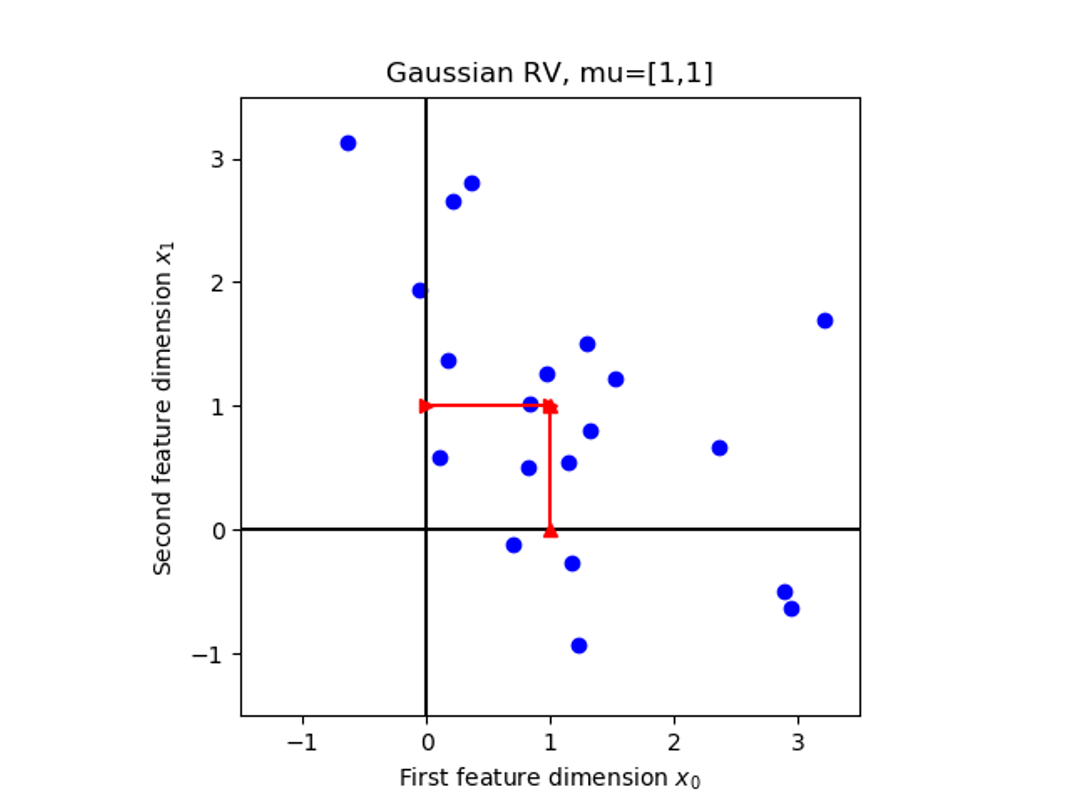
\includegraphics[width=1.9in]{exp/gaussian_vectors.png}
      {\footnotesize\url{https://commons.wikimedia.org/wiki/File:EM-Gaussian-data.svg}}
    \end{block}
  \end{columns}
\end{frame}

\begin{frame}
  \begin{columns}
    \column{2.25in}
    \begin{block}{Maximum Likelihood Parameter Estimation}
      If you differentiate the RHS on the previous slide, and set it
      to zero, you find that the maximum likelihood solution is
      \begin{align*}
        \hat{\mu}_{ML} &= \frac{1}{M}\sum_{m=0}^{M-1}\mathbf{x}_m\\
        \sigma^2_{i,\text{ML}} &= \frac{1}{M}\sum_{m=0}^{M-1}(x_i-\mu_i)^2
      \end{align*}
    \end{block}
    \column{2in}
    \begin{block}{Example: Instances of Gaussian random vectors}
      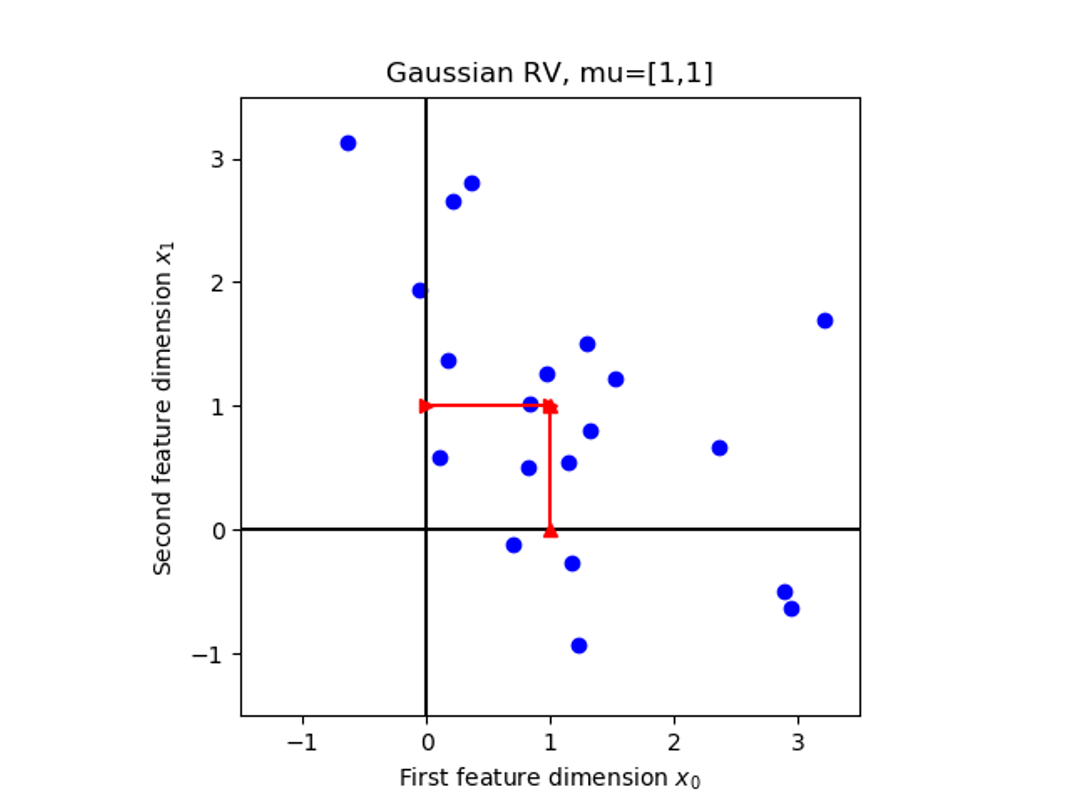
\includegraphics[width=1.9in]{exp/gaussian_vectors.png}
      {\footnotesize\url{https://commons.wikimedia.org/wiki/File:EM-Gaussian-data.svg}}
    \end{block}
  \end{columns}
\end{frame}

\begin{frame}
  \begin{columns}
    \column{2.25in}
    \begin{block}{Sample Mean, Sample Variance}
      The ML estimate of $\sigma_i^2$ is usually too small.  It is better
      to adjust it slightly.  The following are the {\bf unbiased
        estimators} of $\bm{\mu}$ and $\sigma_i^2$, also called the {\bf
        sample mean} and {\bf sample variance}:
      \[
      \bm{\mu}=\frac{1}{M}\sum_{m=0}^{M-1}\mathbf{x}_m
      \]
      \[
      \sigma_i^2=\frac{1}{M-1}\sum_{m=0}^{M-1}(x_i-\mu_i)^2
      \]
    \end{block}
    \column{2in}
    \begin{block}{Example: Instances of Gaussian random vectors}
      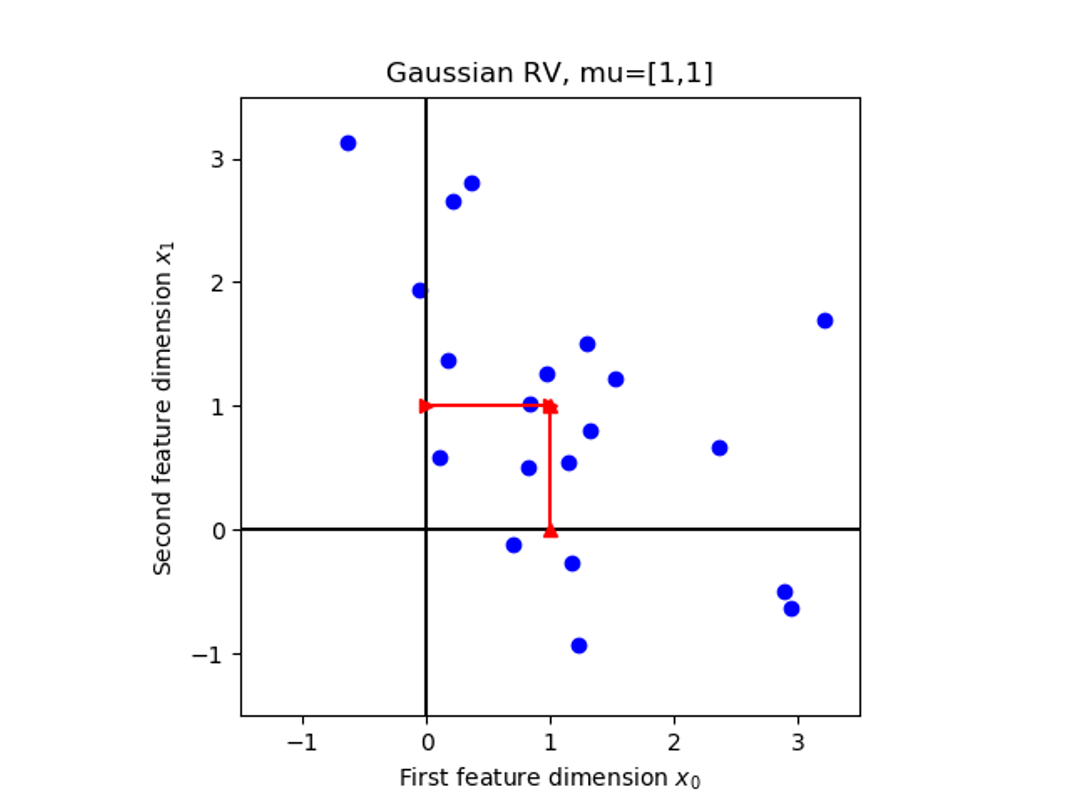
\includegraphics[width=1.9in]{exp/gaussian_vectors.png}
      {\footnotesize\url{https://commons.wikimedia.org/wiki/File:EM-Gaussian-data.svg}}
    \end{block}
  \end{columns}
\end{frame}

\begin{frame}
  \begin{columns}
    \column{2.25in}
    \begin{block}{Sample Mean, Sample Variance}
      \[
      \bm{\mu}=\frac{1}{M}\sum_{m=0}^{M-1}\mathbf{x}_m
      \]
      \[
      \sigma_i^2=\frac{1}{M-1}\sum_{m=0}^{M-1}(\mathbf{x}_m-\bm{\mu})(\mathbf{x}_m-\bm{\mu})^T
      \]
      Sample mean and sample covariance are not the same as real mean
      and real covariance, but we'll use the same letters ($\bm{\mu}$
      and $\bm{\Sigma}$) unless the problem requires us to distinguish.
    \end{block}
    \column{2in}
    \begin{block}{Example: Instances of Gaussian random vectors}
      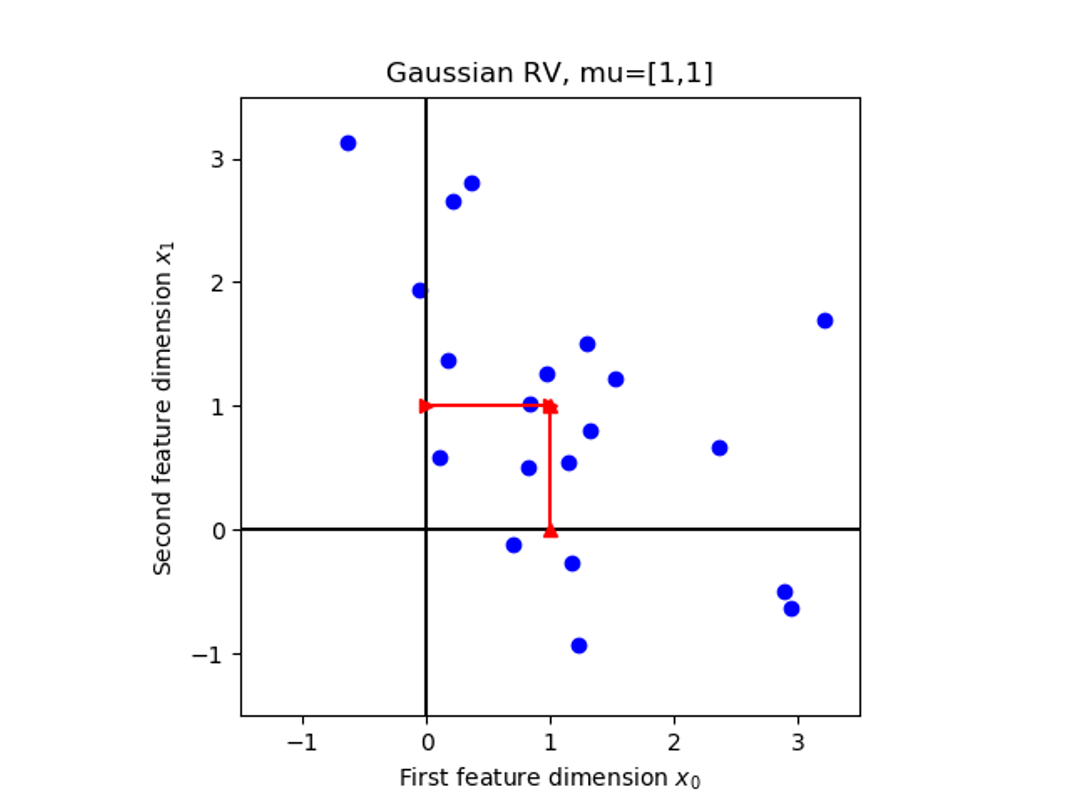
\includegraphics[width=1.9in]{exp/gaussian_vectors.png}
      {\footnotesize\url{https://commons.wikimedia.org/wiki/File:EM-Gaussian-data.svg}}
    \end{block}
  \end{columns}
\end{frame}

%%%%%%%%%%%%%%%%%%%%%%%%%%%%%%%%%%%%%%%%%%%%
\section[Non-Diagonal Covariance]{Vector of Gaussians that are neither independent nor identical}
\setcounter{subsection}{1}

\begin{frame}
  \frametitle{Gaussians with non-diagonal covariance matrix}
  If the dimensions are jointly Gaussian but {\bf not independent} then we
  can still write the multivariate Gaussian as
  \[
  p_{\mathbf{X}}(\mathbf{x})=\frac{1}{(2\pi)^{D/2}|\bm{\Sigma}|^{1/2}}e^{-\frac{1}{2}
    (\mathbf{x}-\bm{\mu})^T\bm{\Sigma}^{-1}(\mathbf{x}-\bm{\mu})}
  \]
  \ldots but now the off-diagonal elements of the
  covariance matrix, $\bm{\Sigma}$, are no longer zero.
  
  \centerline{\includegraphics[height=1in]{exp/dependent_samples.png}\includegraphics[height=1in]{exp/gaussian_copula.png}}
             {\footnotesize\url{https://commons.wikimedia.org/wiki/File:Multinormal_3_true.png},\url{https://commons.wikimedia.org/wiki/File:Gaussian_copula_gaussian_marginals.png}}

\end{frame}

\begin{frame}
  \begin{columns}
    \column{2.25in}
    \begin{block}{Example}
      Suppose that $X_1$ and $X_2$ are Gaussian RVs with means $1$ and
      $-1$, variances $1$ and $4$, and covariance $1$.
      \begin{displaymath}
        \mathbf{x}=\left[\begin{array}{c}1\\-1\end{array}\right]
      \end{displaymath}
      \begin{align*}
        \sigma_1^2 &=E\left[(x_1-\mu_1)^2\right]\\
        &= 1\\
        \sigma_2^2&=E\left[(x_2-\mu_2)^2\right]\\
        &=4\\
        \rho_{1,2}&=E\left[(x_1-\mu_1)(x_2-\mu_2)\right]\\
        &=1
      \end{align*}
    \end{block}
    \column{2in}
    \begin{block}{Example}
      \centerline{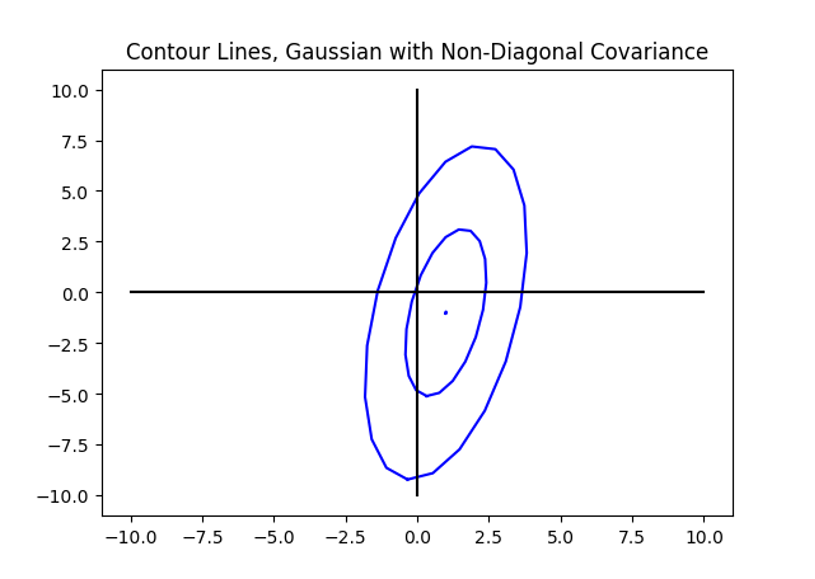
\includegraphics[width=\textwidth]{figs/covariance_example.png}}
    \end{block}
  \end{columns}    
\end{frame}

\begin{frame}
  \begin{columns}
    \column{2.25in}
    \begin{block}{Example}
      Suppose that $X_1$ and $X_2$ are Gaussian RVs with means $1$ and
      $-1$, variances $1$ and $4$, and covariance $1$.
      \begin{displaymath}
        \mathbf{x}=\left[\begin{array}{c}1\\-1\end{array}\right]
      \end{displaymath}
      \begin{align*}
        \bm{\Sigma}&=E\left[(\mathbf{x}-\bm{\mu})(\mathbf{x}-\bm{\mu})^T\right]\\
        &=\left[\begin{array}{cc}1&1\\1&4\end{array}\right]
      \end{align*}
    \end{block}
    \column{2in}
    \begin{block}{Example}
      \centerline{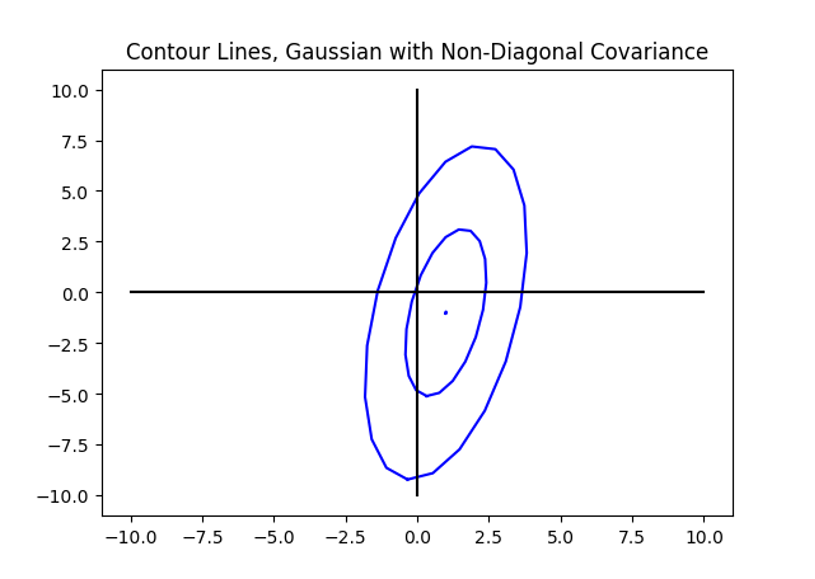
\includegraphics[width=\textwidth]{figs/covariance_example.png}}
    \end{block}
  \end{columns}    
\end{frame}

\begin{frame}
  \frametitle{Determinant and inverse of a $2\times 2$ matrix}

  You should know the determinant and inverse of a $2\times 2$ matrix.  If
  \begin{displaymath}
    \bm{\Sigma}=\left[\begin{array}{cc}a&b\\c&d\end{array}\right]
  \end{displaymath}
  Then $|\bm{\Sigma}|=ad-bc$, and
  \begin{displaymath}
    \bm{\Sigma}^{-1}=\frac{1}{|\bm{\Sigma}|}\left[\begin{array}{cc}d&-b\\-c&a\end{array}\right]
  \end{displaymath}
  If you've never done it before, please prove this formula for
  yourself by multiplying $\bm{\Sigma}^{-1}\bm{\Sigma}$ and
  verifying that the result is the identity matrix.
\end{frame}

\begin{frame}
  \frametitle{Example Multivariate Gaussian}

  The contour lines of our example are the contours along which the
  Mahalanobis distance is equal to a constant:
  \begin{align*}
    &d_{\bm{\Sigma}}(\mathbf{x},\bm{\mu})
    = (\mathbf{x}-\bm{\mu})^T\bm{\Sigma}^{-1}(\mathbf{x}-\bm{\mu})\\
    &= \frac{1}{\sigma_1^2\sigma_2^2-\rho_{1,2}^2}
    [(x_1-\mu_1),(x_2-\mu_2)]
    \left[\begin{array}{cc}\sigma_2^2&-\rho_{1,2}\\-\rho_{1,2}&\sigma_1^2\end{array}\right]
    \left[\begin{array}{c}x_1-\mu_1\\x_2-\mu_2\end{array}\right]\\
    &=\frac{\sigma_2^2}{|\bm{\Sigma}|}(x_1-\mu_1)^2+
    \frac{\sigma_1^2}{|\bm{\Sigma}|}(x_2-\mu_2)^2-
    2\frac{\rho_{1,2}}{|\bm{\Sigma}|}(x_1-\mu_1)(x_2-\mu_2)
  \end{align*}
  This is the formula for an ellipse.
\end{frame}

\begin{frame}
  \begin{columns}
    \column{2.25in}
    \begin{block}{Contours of equal Mahalanobis distance are ellipses}
      \begin{align*}
        &d_{\bm{\Sigma}}(\mathbf{x},\bm{\mu})\\
        &= (\mathbf{x}-\bm{\mu})^T\bm{\Sigma}^{-1}(\mathbf{x}-\bm{\mu})\\
      \end{align*}
    \end{block}
    \column{2in}
    \begin{block}{Example}
      \centerline{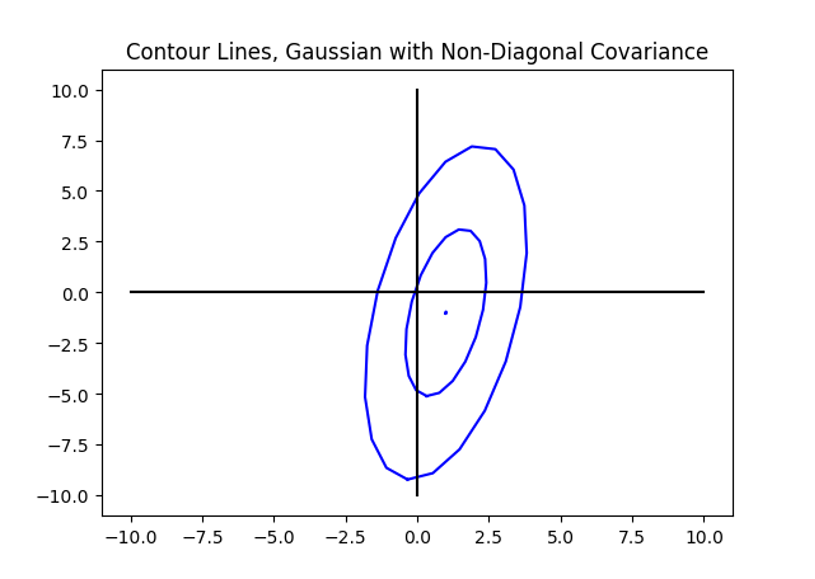
\includegraphics[width=\textwidth]{figs/covariance_example.png}}
    \end{block}
  \end{columns}    
\end{frame}

\begin{frame}
  \frametitle{Maximum Likelihood Parameter Estimation}
  In the real world, we don't know $\bm{\mu}$ and $\bm{\Sigma}$!
  
  If we have a training database ${\mathcal
    D}=\left\{\mathbf{x}_1,\ldots,\mathbf{x}_{M}\right\}$, we can
  estimate $\bm{\mu}$ and $\bm{\Sigma}$ according to
  \begin{align*}
    \left\{\hat\mu_{ML},\hat{\bm{\Sigma}}_{ML}\right\} &= \argmax
    \prod_{m=1}^{M} p(\mathbf{x}_m|\bm{\mu},\bm{\Sigma})\\
    &= \argmax
    \sum_{m=1}^{M} \ln p(\mathbf{x}_m|\bm{\mu},\bm{\Sigma})\\
    \hat{\mu}_{ML} &= \frac{1}{M}\sum_{m=0}^{M-1}\mathbf{x}_m\\
    \hat{\bm{\Sigma}}_{ML} &= \frac{1}{M}\sum_{m=0}^{M-1}(\mathbf{x}_m-\bm{\mu})(\mathbf{x}_m-\bm{\mu})^T
  \end{align*}
\end{frame}

\begin{frame}
  \frametitle{Sample Mean, Sample Covariance}
  The ML estimate of $\bm{\Sigma}$ is usually too small.  It is better
  to adjust it slightly.  The following are the {\bf unbiased
    estimators} of $\bm{\mu}$ and $\bm{\Sigma}$, also called the {\bf
    sample mean} and {\bf sample covariance}:
  \[
  \bm{\mu}=\frac{1}{M}\sum_{m=0}^{M-1}\mathbf{x}_m
  \]
  \[
  \bm{\Sigma}=\frac{1}{M-1}\sum_{m=0}^{M-1}(\mathbf{x}_m-\bm{\mu})(\mathbf{x}_m-\bm{\mu})^T
  \]
\end{frame}

%%%%%%%%%%%%%%%%%%%%%%%%%%%%%%%%%%%%%%%%%%%%
\section[Eigenvectors]{Eigenvectors of the Covariance Matrix}
\setcounter{subsection}{1}


\begin{frame}
  \frametitle{Review: Eigenvalues and eigenvectors of a symmetric matrix}

  The eigenvectors and eigenvalues of a $D\times D$ square matrix,
  $\mathbf{A}$, are the vectors $\mathbf{u}$ and scalars $\lambda$
  such that
  \begin{align*}
    \mathbf{A}\mathbf{u}&=\lambda\mathbf{u}\\
    |\mathbf{A}-\lambda \mathbf{I}|&=0
  \end{align*}
  If $\mathbf{A}$ is symmetric, then we can also multiply from the left:
  \[
  \mathbf{u}^T \mathbf{A} = \lambda\mathbf{u}^T
  \]
\end{frame}

\begin{frame}
  \frametitle{Review: Positive semi-definite matrix}

  A positive-semidefinite matrix (we write $\mathbf{A}\succcurlyeq 0$)
  is one such that, for every vector $\mathbf{u}\in\Re^D$,
  \begin{displaymath}
    \mathbf{u}^T\mathbf{A}\mathbf{u} \ge 0
  \end{displaymath}
  Every $D\times D$ matrix has $D$ eigenvalues.  A positive
  semi-definite matrix is also guaranteed to have $D$ eigenvectors,
  though some of them may not be uniquely specified (if eigenvalues
  repeat, then the corresponding eigenvectors can be any orthonormal
  vectors spanning the corresponding subspace).
\end{frame}

\begin{frame}
  \frametitle{Symmetric positive semi-definite matrices: eigenvectors are orthonormal}

  If $\mathbf{A}$ is symmetric and positive-semidefinite, then
  \begin{align*}
    (\mathbf{u}_i^T\mathbf{A})\mathbf{u}_j&=(\lambda_i\mathbf{u}_i)^T\mathbf{u}_j\\
    \mathbf{u}_i^T(\mathbf{A}\mathbf{u}_j)&=\mathbf{u}_i^T(\lambda_j\mathbf{u}_j)
  \end{align*}
  These can only both be true if either $\lambda_i=\lambda_j$ or
  $\mathbf{u}_i^T\mathbf{u}_j=0$.  By defining $|\mathbf{u}_i|=1$, we
  can choose eigenvectors such that
  \begin{displaymath}
    \mathbf{u}_i^T\mathbf{u}_j=\left\{\begin{array}{ll}
    1 & i=j\\
    0 & i\ne j
    \end{array}\right.
  \end{displaymath}
  If we define the eigenvectors matrix as $\mathbf{U}=[\mathbf{u}_1,\ldots,\mathbf{u}_D]$, then
  \begin{displaymath}
    \mathbf{U}^T\mathbf{U}=\mathbf{I}
  \end{displaymath}
\end{frame}
    
\begin{frame}
  \frametitle{Symmetric positive semi-definite matrices: eigenvectors diagonalize the matrix}

  If $\mathbf{A}$ is symmetric and positive-semidefinite, then
  \[
  \mathbf{u}_i^T\mathbf{A}\mathbf{u}_j=
  \mathbf{u}_i^T(\lambda_j\mathbf{u}_j)=\lambda_j\mathbf{u}_i^T\mathbf{u}_j
  =\begin{cases}\lambda_j,&i=j\\0,&i\ne j\end{cases}
  \]
  In other words, the eigenvectors orthogonalize $\mathbf{A}$:
  \[
  \mathbf{U}^T\mathbf{A}\mathbf{U} = \bm{\Lambda}
  \]
  \ldots where $\bm{\Lambda}$ is the diagonal matrix of eigenvalues:
  \[
  \bm{\Lambda}=
  \left[\begin{array}{ccc}\lambda_1&0&0\\0&\ldots&0\\0&0&\lambda_{D}\end{array}\right]
  \]
\end{frame}


\begin{frame}
  \frametitle{A symmetric positive semidefinite matrix is the weighted sum of its eigenvectors}

  The previous slide showed that
  $\bm{\Lambda}=\mathbf{U}^T\mathbf{A}\mathbf{U}$.  Wrap that
  whole equation in $\mathbf{U}\cdots\mathbf{U}^T$, and you get:
  \[
  \mathbf{U}\bm{\Lambda}\mathbf{U}^T=
  \mathbf{U}\mathbf{U}^T\bm{A}\mathbf{U}\mathbf{U}^T =\mathbf{A}
  \]
  In other words, any symmetric positive semidefinite matrix can be
  expanded as:
  \[
  \mathbf{A}=
  \left[\mathbf{u}_1,\ldots,\mathbf{u}_{D}\right]
  \left[\begin{array}{ccc}\lambda_1&0&0\\0&\ldots&0\\0&0&\lambda_{D}\end{array}\right]  
  \left[\begin{array}{c}\mathbf{u}_1^T\\\vdots\\\mathbf{u}_{D}^T\end{array}\right]=
  \sum_{d=1}^{D}\lambda_d \mathbf{u}_d\mathbf{u}_d^T
  \]
\end{frame}

\begin{frame}
  \frametitle{Summary: properties of symmetric positive semidefinite
    matrices}

  If $\mathbf{A}$ is any positive semidefinite matrix, then:
  \[
  \mathbf{A}=\mathbf{U}\bm{\Lambda} \mathbf{U}^T,
  \]
  and
  \[
  \bm{\Lambda} = \mathbf{U}^T\mathbf{A}\mathbf{U},
  \]
  where $\bm{\Lambda}$ is diagonal and $\mathbf{U}$ is orthonormal:
  \[
  \mathbf{U}\mathbf{U}^T=\mathbf{U}^T\mathbf{U}=\mathbf{I}
  \]
\end{frame}

\begin{frame}
  \frametitle{The covariance matrix is symmetric}

  Covariance is symmetric:
  \begin{displaymath}
    \rho_{1,2}=E\left[(x_1-\mu_1)(x_2-\mu_2)\right]=\rho_{2,1}
  \end{displaymath}
  \ldots and therefore the covariance matrix is symmetric:
  \begin{align*}
    \bm{\Sigma}&=E\left[(\mathbf{x}-\bm{\mu})(\mathbf{x}-\bm{\mu})^T\right]\\
    &=
    \left[\begin{array}{cccc}
        \sigma_1^2&\rho_{1,2}&\cdots&\rho_{1,M}\\
        \rho_{1,2}&\sigma_2^2&\cdots&\rho_{2,M}\\
        \vdots&\vdots&\ddots&\vdots\\
        \rho_{1,M}&\rho_{2,M}&\cdots&\sigma_M^2
      \end{array}\right]
  \end{align*}
\end{frame}

\begin{frame}
  \frametitle{The covariance matrix is positive semidefinite}

  The covariance matrix is also positive semidefinite. Here's a
  proof. Suppose we multiply it by any vector, $\mathbf{u}$:
  \begin{align*}
    &\mathbf{u}^T\bm{\Sigma}\mathbf{u}\\
    &=\mathbf{u}^TE\left[(\mathbf{x}-\bm{\mu})(\mathbf{x}-\bm{\mu})^T\right]\mathbf{u}\\
    &=E\left[\mathbf{u}^T(\mathbf{x}-\bm{\mu})(\mathbf{x}-\bm{\mu})^T\mathbf{u}\right]\\
    &=E\left[\left(\mathbf{u}^T(\mathbf{x}-\bm{\mu})\right)^2\right]\ge 0
  \end{align*}
\end{frame}

\begin{frame}
  \frametitle{Summary: properties of the covariance matrix}

  If $\bm{\Sigma}$ is the covariance matrix of any Gaussian, then
  \[
  \bm{\Sigma}=\mathbf{U}\bm{\Lambda} \mathbf{U}^T,
  \]
  and
  \[
  \bm{\Lambda} = \mathbf{U}^T\bm{\Sigma}\mathbf{U},
  \]
  where $\bm{\Lambda}$ is diagonal and $\mathbf{U}$ is orthonormal:
  \[
  \mathbf{U}\mathbf{U}^T=\mathbf{U}^T\mathbf{U}=\mathbf{I}
  \]
\end{frame}

%%%%%%%%%%%%%%%%%%%%%%%%%%%%%%%%%%%%%%%%%%%%
\section[NN]{Nearest-Neighbors Classifier}
\setcounter{subsection}{1}

\begin{frame}
  \frametitle{How do you classify an image?}

  Suppose we have a test image, $\mathbf{x}_{\mbox{test}}$.  We want to figure out:
  who is this person?

  \begin{centering}
    \begin{block}{\bf Test Datum $\mathbf{x}_{\mbox{test}}$:}
      
\includegraphics[width=1.5in]{exp/Megawati_Sukarnoputri_0002.jpg}
    \end{block}
  \end{centering}
  
\end{frame}
    
\begin{frame}
  \frametitle{Training Data?}
  In order to classify the test image, we need some training data.
  For example, suppose we have the following four images in our
  training data.  Each image, $\mathbf{x}_m$, comes with a label, $\ell_m$,
  which is just a string giving the name of the individual.
  \begin{columns}
    \column{1.05in}
    \begin{block}{\bf Training Datum: $\ell_1=$Colin Powell:}
      $\mathbf{x}_0=$
      
\includegraphics[width=1in]{exp/Colin_Powell_0001.jpg}
    \end{block}
    \column{1.05in}
    \begin{block}{\bf Training Datum $\ell_2=$Gloria Arroyo:}
      $\mathbf{x}_1=$
      
\includegraphics[width=1in]{exp/Gloria_Macapagal_Arroyo_0001.jpg}
    \end{block}
    \column{1.05in}
    \begin{block}{\bf Training Datum $\ell_3=$Megawati Sukarnoputri:}
      $\mathbf{x}_2=$
      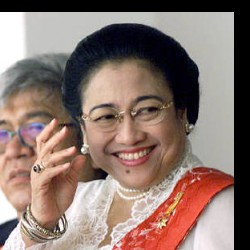
\includegraphics[width=1in]{exp/Megawati_Sukarnoputri_0001.jpg}
    \end{block}
    \column{1.05in}
    \begin{block}{\bf Training Datum $\ell_4=$Tony Blair:}
      $\mathbf{x}_3=$
      
\includegraphics[width=1in]{exp/Tony_Blair_0001.jpg}
    \end{block}
  \end{columns}
\end{frame}
    
\begin{frame}
  \frametitle{Nearest Neighbors Classifier}

  A ``nearest neighbors classifier'' makes the following
  guess: the test vector is an image of the same person as the
  closest training vector:
  \[
  \hat{\ell}_{\mbox{test}} = \ell_{m^*},~~~
  m^*=\argmin_{m=1}^{M}\Vert\mathbf{x}_m-\mathbf{x}_{\mbox{test}}\Vert
  \]
  where ``closest,'' here, means Euclidean distance:
  \[
  \Vert\mathbf{x}_m-\mathbf{x}_{\mbox{test}}\Vert =
  \sqrt{\sum_{d=1}^{D} (x_{m,d}-x_{\mbox{test},d})^2}
  \]
\end{frame}

\begin{frame}
  \frametitle{Improved Nearest Neighbors: Eigenface}

  \begin{itemize}
    \item 
      The problem with nearest-neighbors is that subtracting one image
      from another, pixel-by-pixel, results in a measurement that is
      dominated by noise.
    \item 
      We need a better measurement.
    \item
      The solution is to find a signal representation, $\mathbf{y}_m$,
      such that $\mathbf{y}_m$ summarizes the way in which $\mathbf{x}_m$
      differs from other faces.
    \item
      If we find $\mathbf{y}_m$ using principal components analysis, then
      $\mathbf{y}_m$ is called an ``eigenface'' representation.
  \end{itemize}
\end{frame}
  

%%%%%%%%%%%%%%%%%%%%%%%%%%%%%%%%%%%%%%%%%%%%
\section[PCA]{Principal Components}
\setcounter{subsection}{1}

\begin{frame}
  \frametitle{Sample covariance}
  Remember that the sample covariance is defined as:
  \begin{align*}
    \bm{\Sigma}&=\frac{1}{M-1}\sum_{m=0}^{M-1}(\mathbf{x}_m-\bm{\mu})(\mathbf{x}_m-\bm{\mu})^T\\
    &=\frac{1}{M-1}\mathbf{X}\mathbf{X}^T
  \end{align*}
  \ldots where $\mathbf{X}$ is the centered data matrix,
  \[
  \mathbf{X}=\left[\mathbf{x}_1-\bm{\mu},\ldots,\mathbf{x}_{M}-\bm{\mu}\right]
  \]
\end{frame}

\begin{frame}
  \begin{columns}
    \column{1.75in}
    \begin{block}{Centered data matrix}
      \[
      \mathbf{X}=\left[
        \mathbf{x}_1-\bm{\mu},\ldots,\mathbf{x}_{M}-\bm{\mu}\right]
      \]
    \end{block}
    \column{2.625in}
    \begin{block}{Examples of $\mathbf{x}_m-\bm{\mu}$}
      \includegraphics[width=2.1in]{exp/sample_covariance.png}
      {\footnotesize\url{https://commons.wikimedia.org/wiki/File:PCA_Pires.jpg}}
    \end{block}
  \end{columns}
\end{frame}

\begin{frame}
  \begin{columns}
    \column{1.75in}
    \begin{block}{Principal component axes}
      
      The eigenvectors of the sample covariance are called the
      principal component axes, or principal component directions.
    \end{block}
    \column{2.625in}
    \begin{block}{Principal component axes}
      \includegraphics[width=\textwidth]{exp/GaussianScatterPCA.png}
      {\footnotesize\url{https://commons.wikimedia.org/wiki/File:GaussianScatterPCA.svg}}
    \end{block}
  \end{columns}
\end{frame}

\begin{frame}
  \frametitle{Principal components}

  The principal component analysis of $\mathbf{x}_m$ is the vector
  $\mathbf{y}_m=\mathbf{U}^T(\mathbf{x}_m-\bm{\mu})$, where $\mathbf{U}$
  are the eigenvectors of the covariance.
  We can compute the principal components analysis (PCA) of every
  vector in the training dataset by computing
  \begin{align*}
    \mathbf{Y}&=[\mathbf{y}_1,\ldots,\mathbf{y}_M]\\
    &=\mathbf{U}^T\mathbf{X}
  \end{align*}
  Now let's ask: what is the sample covariance of the PCA vectors?
  The sample covariance is defined as:
  \begin{align*}
    \frac{1}{M-1}\mathbf{Y}\mathbf{Y}^T
    &= \frac{1}{M-1}\mathbf{U}^T\mathbf{X}\mathbf{X}^T\mathbf{U}\\
    &= \mathbf{U}^T\bm{\Sigma}\mathbf{U}\\
    &= \bm{\Lambda}
  \end{align*}
  So the covariance of $\mathbf{Y}$ is a diagonal matrix,
  $\bm{\Lambda}$.
\end{frame}

\begin{frame}
  \frametitle{Principal components}
  
  The vector $\mathbf{y}_m$ is called the \textbf{principal components
    analysis} (PCA) of $\mathbf{x}_m$.  Let's examine its structure a
  little.
  \begin{align*}
    \mathbf{y}_m
    &= \mathbf{U}^T(\mathbf{x}_m-\bm{\mu}) 
    &= \left[\begin{array}{c}\mathbf{u}_1^T\\\vdots\\\mathbf{u}_D^T\end{array}\right]
    (\mathbf{x}_m-\bm{\mu})
    &= \left[\begin{array}{c}\mathbf{u}_1^T(\mathbf{x}_m-\bm{\mu})\\
        \vdots\\
        \mathbf{u}_D^T(\mathbf{x}_m-\bm{\mu})\end{array}\right]
  \end{align*}
  We can say that the $j^{\text{th}}$ principal component of $\mathbf{x}_m$ is
  \begin{displaymath}
    y_{j,m} = \mathbf{u}_j^T(\mathbf{x}_m-\bm{\mu})
  \end{displaymath}
\end{frame}

\begin{frame}
  \begin{columns}
    \column{1.75in}
    \begin{block}{Orthogonal projection}

      Remember that the eigenvectors were defined to have unit length,
      therefore $y_{j,m}=\mathbf{u}_j(\mathbf{x}_m-\bm{\mu})$ is
      the orthogonal projection of $\mathbf{x}_m-\bm{\mu}$ onto
      the $j^{\text{th}}$ principal component direction.
    \end{block}
    \column{2.625in}
    \begin{block}{Principal component axes}
      \includegraphics[width=\textwidth]{exp/orthogonal_projection.png}
      {\footnotesize\url{https://commons.wikimedia.org/wiki/File:Orthogonal_Projection_qtl1.svg}}
    \end{block}
  \end{columns}
\end{frame}

\begin{frame}
  \begin{columns}
    \column{1.75in}
    \begin{block}{Principal components = Orthonormal projection onto principal component directions}

      Remember that the eigenvector matrix is orthonormal,
      therefore $\mathbf{y}=\mathbf{U}^T(\mathbf{x}_m-\bm{\mu})$ is
      just an expression of $\mathbf{x}_m-\bm{\mu}$ in a
      new set of axes.   This operation is sometimes called ``rotation.''
    \end{block}
    \column{2.625in}
    \begin{block}{}
      \centerline{\animategraphics[loop,controls,width=\textwidth]{10}{exp/rotation-}{0}{152}}
      {\footnotesize\url{https://commons.wikimedia.org/wiki/File:Diagonalization_as_rotation.gif}}
    \end{block}
  \end{columns}
\end{frame}


\begin{frame}
  \frametitle{The principal components are linearly independent}

  Suppose that $\mathbf{x}$ is a Gaussian random vector:
  \begin{align*}
    p_X(\mathbf{x})
    &=\frac{1}{\sqrt{|2\pi\bm{\Sigma}|}}
    e^{-\frac{1}{2}(\mathbf{x}-\bm{\mu})^T\bm{\Sigma}^{-1}(\mathbf{x}-\bm{\mu})}\\
    &=\frac{1}{\sqrt{|2\pi\mathbf{U}\bm{\Lambda}\mathbf{U}^T|}}
    e^{-\frac{1}{2}(\mathbf{x}-\bm{\mu})^T\mathbf{U}\bm{\Lambda}^{-1}\mathbf{U}^T(\mathbf{x}-\bm{\mu})}\\
    &=\frac{1}{\sqrt{|2\pi\bm{\Lambda}|}}
    e^{-\frac{1}{2}\mathbf{y}^T\bm{\Lambda}^{-1}\mathbf{y}}\\
    &= \prod_{i=1}^D \frac{1}{\sqrt{2\pi\lambda_i}}
    e^{-\frac{1}{2}\frac{y_i^2}{\lambda_i}}
  \end{align*}
  So if $\mathbf{x}$ is a Gaussian random vector, then the principal
  components are independent zero-mean Gaussian random variables with
  variances of $\lambda_i$.
\end{frame}
  
\begin{frame}
  \frametitle{Principal components are uncorrelated, and PC with
    larger eigenvalues have more energy}

  In the following figure, notice that (1) the principal components
  are uncorrelated with one another, (2) the eigenvalues have been
  sorted so that $\lambda_0>\lambda_1>\lambda_2$ and so on. With this
  sorting, you see that the the first PC has the biggest
  variance:

  \centerline{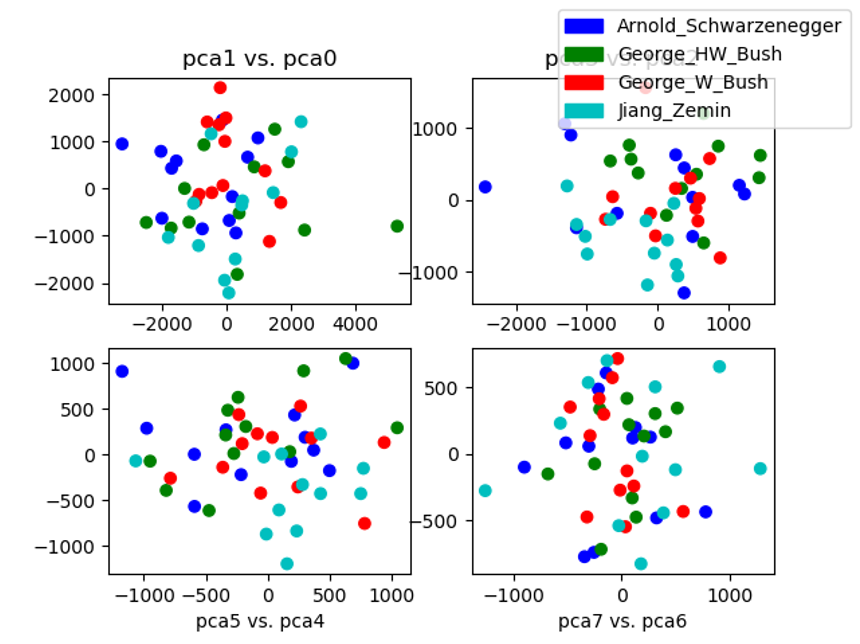
\includegraphics[height=2in]{figs/pca_samples.png}}
\end{frame}

%%%%%%%%%%%%%%%%%%%%%%%%%%%%%%%%%%%%%%%%%%%%
\section[PCA Features]{Using PCA as a compressed representation of the data}
\setcounter{subsection}{1}

\begin{frame}
  \frametitle{Feature embedding}

  \begin{itemize}
  \item Suppose $\mathbf{x}$ is a vector we'd like to classify.
    \begin{itemize}
    \item It has very high dimension, e.g., 6 million.
    \item High-dimensional classifiers are hard to learn.
    \item Probably most of the features are redundant.
    \end{itemize}
  \item Let's learn an embedding $\mathbf{z}=f(\mathbf{x})$ such that:
    \begin{itemize}
    \item $\mathbf{z}$ has low dimension, e.g., 1000
    \item $\mathbf{z}$ contains the important information from $\mathbf{x}$
    \end{itemize}
  \end{itemize}
\end{frame}

\begin{frame}
  \frametitle{Measuring ``importance'' as ``variance''}

  There are many ways to formulate the problem of finding the
  important information in $\mathbf{x}$.  One of the simplest methods
  that works well is to find $\mathbf{z}=[z_1,\ldots,z_K]^T$, $K\ll
  D$, such that:
  \begin{itemize}
  \item Each $z_i$ is just an orthogonal projection of $\mathbf{x}$, i.e., 
    $z_i=\mathbf{f}_i^T(\mathbf{x}-\bm{\mu})$, where $|\mathbf{f}_i|=1$.
  \item Each $z_i$ is uncorrelated with all the others,
    $E\left[z_iz_j\right]=0$.
  \item Given those constraints, it makes sense to choose $z_i$ to
    capture as much of the sample variance of $\mathbf{x}$ as
    possible, in other words, we want:
  \end{itemize}
  \begin{displaymath}
    \mathbf{F} = \argmax\sum_{m=1}^M\sum_{i=1}^K z_{i,m}^2
  \end{displaymath}
  \begin{displaymath}
    \text{such that:}~~\mathbf{z}_m=\mathbf{F}^T(\mathbf{x}_m-\bm{\mu}),
    \mathbf{F}\in\Re^{D\times K},~~\mathbf{F}^T\mathbf{F}=\mathbf{I},
    \sum_{m=1}^Mz_{i,m}z_{j,m}=0
  \end{displaymath}
\end{frame}

\begin{frame}
  \frametitle{PCA = Maximum-variance linear feature embedding}

  We have decided that we want to maximize $\sum_m\sum_i z_{i,m}^2$ subject to the
  following constraints:
  \begin{displaymath}
    \mathbf{z}_m=\mathbf{F}^T(\mathbf{x}_m-\bm{\mu}),
    \mathbf{F}\in\Re^{D\times K},~~\mathbf{F}^T\mathbf{F}=\mathbf{I},
    \sum_{m=1}^Mz_{i,m}z_{j,m}=0
  \end{displaymath}
  All of these constraints are satisfied if we set the feature
  vectors, $\mathbf{f}_i$, equal to any subset of the eigenvectors,
  $\mathbf{u}_i$.  The eigenvectors that maximize $\sum_m\sum_iz_{i,m}^2$
  are those associated with the largest eigenvalues:
  \begin{align*}
    \frac{1}{M-1}\sum_{m=1}^M\sum_{i=1}^K z_{i,m}^2 = \sum_{i=1}^K \lambda_i
  \end{align*}
\end{frame}

\begin{frame}
  \frametitle{Energy  spectrum=Fraction of energy explained}
  The ``energy spectrum'' is energy as a function of
  basis vector index.  There are a few ways we could define it,
  but one useful definition is:
  \begin{align*}
    E[k] &=\frac{\sum_{m=1}^{M}\sum_{i=1}^{k}y_{i,m}^2}
    {\sum_{m=1}^{M}\sum_{i=1}^{D}y_{i,m}^2}\\
    &=\frac{\sum_{i=1}^{k}\lambda_i}{\sum_{i=1}^{D}\lambda_i}
  \end{align*}
  In words, $E[k]$ is the fraction of the sample variance that is captured by
  a feature embedding consisting of the first $k$ principal components.
\end{frame}

\begin{frame}
  \frametitle{Energy  spectrum=Fraction of energy explained}
  \centerline{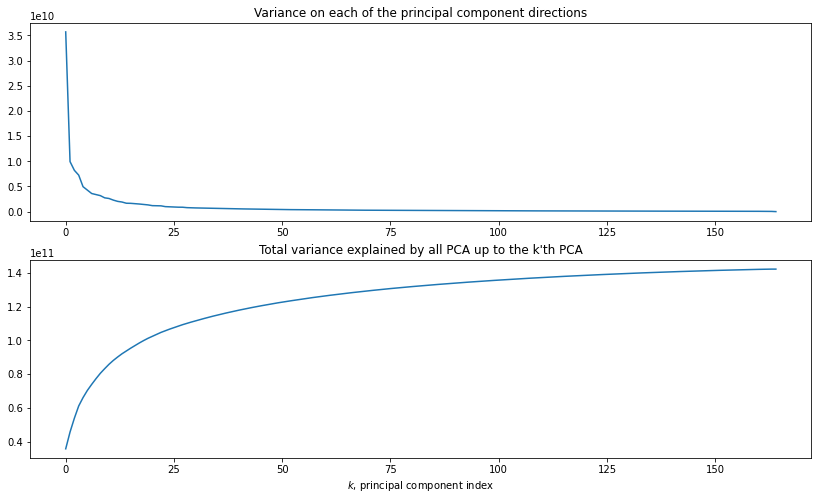
\includegraphics[height=3in]{figs/energy_spectrum.png}}
\end{frame}


%%%%%%%%%%%%%%%%%%%%%%%%%%%%%%%%%%%%%%%%%%%%
\section[Gram]{Computational Considerations: Gram matrix, SVD}
\setcounter{subsection}{1}

\begin{frame}
  \begin{columns}
    \column{2.125in}
    \begin{block}{Gram matrix}
      \begin{itemize}
      \item $\mathbf{S}=\mathbf{X}\mathbf{X}^T$ is usually called the
        sum-of-squares matrix.  $\frac{1}{M-1}\mathbf{S}$
        is the sample covariance.
      \item $\mathbf{G}=\mathbf{X}^T\mathbf{X}$ is called the gram matrix.
        Its $(i,j)^{\textrm{th}}$ element is the dot product between
        the $i^{\textrm{th}}$ and $j^{\textrm{th}}$ data samples:
        \[
        g_{i,j}=(\mathbf{x}_i-\bm{\mu})^T(\mathbf{x}_j-\bm{\mu})
        \]
      \end{itemize}
    \end{block}
    \column{2.125in}
    \begin{block}{Gram matrix $g_{01}=(\mathbf{x}_0-\bm{\mu})^T(\mathbf{x}_1-\bm{\mu})$}
      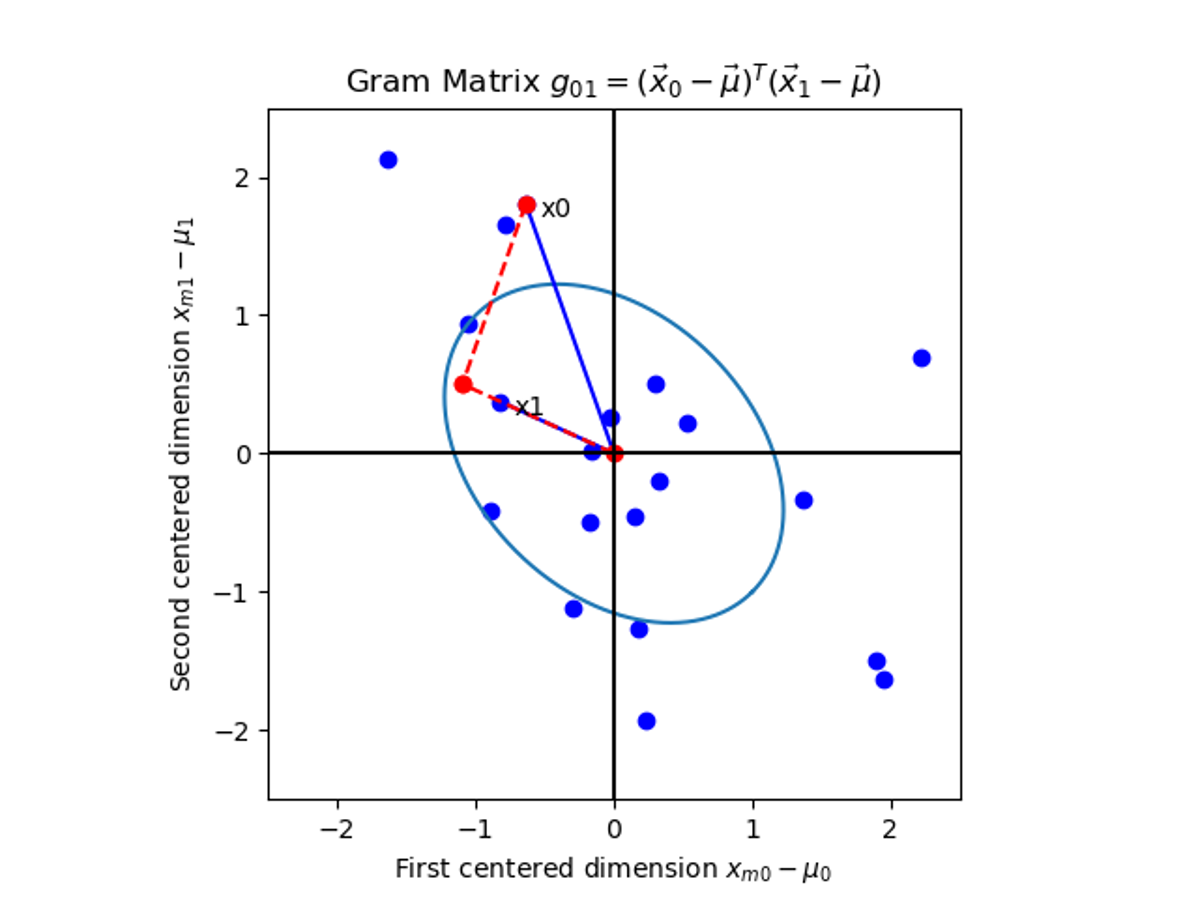
\includegraphics[width=2.1in]{figs/gram_matrix.png}
    \end{block}
  \end{columns}
\end{frame}

\begin{frame}
  \begin{columns}
    \column{2.125in}
    \begin{block}{Eigenvectors of the Gram matrix}
      $\mathbf{G}$ is also symmetric and positive
      semidefinitex!  So it has orthonormal eigenvectors:
      \[
      \mathbf{G}=\mathbf{V}\bm{\Lambda} \mathbf{V}^T
      \]
      \[
      \mathbf{V}\mathbf{V}^T=\mathbf{V}^T\mathbf{V}=\mathbf{I}
      \]
      {\bf Surprising Fact:} $\mathbf{G}$ and $\mathbf{S}$ have the
      same eigenvalues, but different eigenvectors ($\mathbf{U}$
      vs. $\mathbf{V}$).  For this part of the lecture, let's say that
      $\bm{\Lambda}$ are the eigenvalues of the sum-of-squares matrix,
      which are also the eigenvalues of the gram matrix.
    \end{block}
    \column{2.125in}
    \begin{block}{Gram matrix $g_{1,2}=(\mathbf{x}_1-\bm{\mu})^T(\mathbf{x}_2-\bm{\mu})$}
      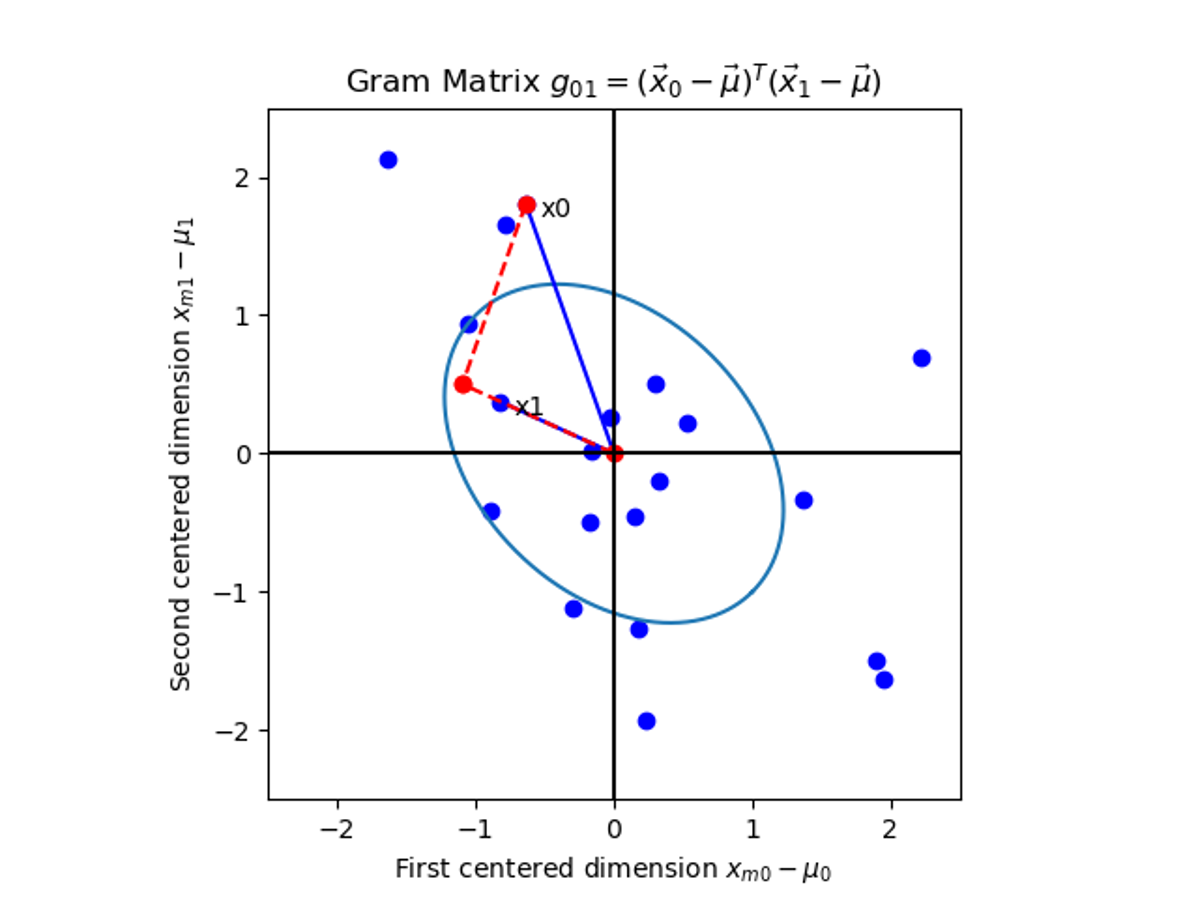
\includegraphics[width=2.1in]{figs/gram_matrix.png}
    \end{block}
  \end{columns}
\end{frame}

\begin{frame}
  \frametitle{Why the Gram matrix is useful:}

  Suppose that $D\sim 240000$ pixels per image, but $M\sim
  240$ different images.  Then,
  \begin{itemize}
  \item $\mathbf{S}$ is a $240000\times 240000$ matrix, and finding
    its eigenvectors is an $\mathcal{O}\left\{(240000)^3\right\}$
    operation.
  \item $\mathbf{G}$ is a $240\times 240$ matrix, and finding its
    eigenvectors is an $\mathcal{O}\left\{(240000)^3\right\}$
    operation.
  \end{itemize}
\end{frame}

\begin{frame}
  \frametitle{Singular Value Decomposition}
  
  Suppose that $\mathbf{X}\in\Re^{D\times M}$ and
  \begin{itemize}
  \item $\mathbf{V}=[\mathbf{v}_1,\ldots,\mathbf{v}_D]$ are the
    eigenvectors of $\mathbf{G}=\mathbf{X}^T\mathbf{X}$, and
    $\lambda_i$ are its eigenvalues, of which at most $\min(M,K)$ are
    nonzero.
  \item $\mathbf{U}=[\mathbf{u}_1,\ldots,\mathbf{u}_M]$ are the
    eigenvectors of $\mathbf{S}=\mathbf{X}\mathbf{X}^T$, and
    $\lambda_i$ are its eigenvalues, of which at most $\min(M,K)$ are
    nonzero.  Then:
  \end{itemize}
  \begin{displaymath}
    \mathbf{X}=\mathbf{U}\bm{\Lambda}^{1/2}\mathbf{V}^T,
  \end{displaymath}
  where $\bm{\Lambda}^{1/2}$ is a $D\times M$ diagonal matrix with
  the singular values, $\lambda_i^{1/2}$, on the diagonal.
\end{frame}

\begin{frame}
  \frametitle{How to find the principal components from the eigenvectors of the gram matrix}

  \begin{itemize}
  \item Suppose you've computed the eigenvectors of the gram matrix,
    $\mathbf{V}$, and you want to find the principal component
    directions, $\mathbf{U}$.  How can you do that?
  \item Answer: multiply by the data matrix, $\mathbf{X}$, then divide
    by the singular values:
  \end{itemize}
  \begin{align*}
    \mathbf{X}\mathbf{V}\bm{\Lambda}^{-1/2}
    &=\mathbf{U}\bm{\Lambda}^{1/2}\mathbf{V}^T\mathbf{V}\bm{\Lambda}^{-1/2}\\
    &=\mathbf{U}\bm{\Lambda}^{1/2}\bm{\Lambda}^{-1/2}\\
    &=\mathbf{U}
  \end{align*}
\end{frame}

\begin{frame}
  \frametitle{How to find the principal components directly from the data matrix, without ever computing either the sample covariance matrix or the gram matrix}

  Use {\tt np.linalg.svd(X)}.  This function will:
  \begin{itemize}
  \item Check whether $\mathbf{X}$ has more rows or more columns.
  \item Depending on the answer, find eigenvalues and eigenvectors of
    either $\mathbf{X}^T\mathbf{X}$ or $\mathbf{X}\mathbf{X}^T$.
  \item Find the other set of eigenvectors using one of the following two equations:
  \end{itemize}
  \begin{align*}
    \mathbf{U}&=\mathbf{X}\mathbf{V}\bm{\Lambda}^{-1/2},~~~\text{or}\\
    \mathbf{V}&=\mathbf{X}^T\mathbf{U}\bm{\Lambda}^{-1/2}\\
  \end{align*}
\end{frame}

%%%%%%%%%%%%%%%%%%%%%%%%%%%%%%%%%%%%%%%%%%%%
\section[Summary]{Summary}
\setcounter{subsection}{1}

\begin{frame}
  \frametitle{Summary}
  \begin{itemize}
  \item Symmetric positive semidefinite matrices:
    \[
    \mathbf{A}=\mathbf{U}\bm{\Lambda} \mathbf{U}^T,~~\mathbf{U}^T\mathbf{A}\mathbf{U}=\bm{\Lambda},~~\mathbf{U}^T\mathbf{U}=\mathbf{U}\mathbf{U}^T=\mathbf{I}
    \]
  \item Centered dataset:
    \[
    \mathbf{X} = \left[\mathbf{x}_1-\bm{\mu},\ldots,\mathbf{x}_{M}-\bm{\mu}\right]
    \]
  \item Singular value decomposition:
    \[
    \mathbf{X} = \mathbf{U}\bm{\Lambda}^{1/2}\mathbf{V}^T
    \]
    where $\mathbf{V}$ are eigenvectors of the gram matrix,
    $\mathbf{U}$ are eigenvectors of the covariance matrix, and
    $\bm{\Lambda}$ are their shared eigenvalues.
  \item The principal components are the first $K$ elements of
    $\mathbf{y}=\mathbf{U}^T(\mathbf{x}-\bm{\mu})$.  Principal
    component analysis maximizes the variance of $\mathbf{y}$ subject
    to the constraints that each dimension is a linearly independent
    orthonormal projection of $\mathbf{x}$.
  \end{itemize}
\end{frame}


\end{document}
